%%%%%%%%%%%%%%%%%%%%%%%%%%%%%%%%%%%%%%%%%%%%%%%%
\input{./format/preamble.ltx} 

%%%%%%%%%%%%%%%%%%%%%%%%%%%%%%%%%%%%%%%%%%%%%%%%
% as needed, comment the following lines by prefixing the percent sign at the start of the line

\PutLineNumberstrue % comment only if line numbers will not be put at the left side margin; this also will turn off certain  preparation guides 

\Figurestrue % comment only if figures will not be rendered 

\GroupIDtrue % comment if no group ID

\ResultDiscusstrue % comment to disable results and discussions

\Conctrue % comment to disable conclusions

\Finishedtrue % comment only if you will not be printing your manuscript prior to final hard binding, i.e. you are not told by your thesis adviser that you have passed, and you have no submitted the requirements

%\Gradtrue % comment to disable graduate school format

\PhDtrue % comment to disable PhD dissertation format

\PubListtrue % comment to disable publication list

\Vitatrue % comment to disable author(s) vita

\Indextrue % comment to disable index 

%%%%%%%%%%%%%%%%%%%%%%%%%%%%%%%%%%%%%%%%%%%%%%%%
% document IDs

\newcommand{\documentType}{Thesis} % specify if dissertation, thesis, project, dissertation proposal, thesis proposal, project proposal 
\newcommand{\college}{Gokongwei College of Engineering}
\newcommand{\department}{Department of Electronics and Communications Engineering} 
\newcommand{\degreeType}{Bachelor of Science} 
\newcommand{\degree}{Electronics and Communications Engineering}
\newcommand{\degreeAbbrv}{BS-ECE}

\newcommand{\documentAdviserTitle}{Engr.} 
\newcommand{\documentAdviser}{Donabel D. Abuan}

\newcommand{\examinerChairTitle}{Dr.} 
\newcommand{\examinerChair}{Amado Z. Hernandez}

% Sort in alphabetically ascending manner the surnames of the examiners
\newcommand{\examinerATitle}{Dr.} 
\newcommand{\examinerA}{Aaron F. Africa}

\newcommand{\examinerBTitle}{Engr.} 
\newcommand{\examinerB}{Argel A. Bandala}

% Note that \examinerC and \examinerD only applies for PhD dissertations
\newcommand{\examinerCTitle}{Engr.} 
\newcommand{\examinerC}{Oswald Sapang}

\newcommand{\examinerDTitle}{Engr.} 
\newcommand{\examinerD}{Roderick Yap}

\newcommand{\deanTitle}{Dr.} 
\newcommand{\deanName}{Rosemary R. Seva}

\newcommand{\groupID}{ESG-04} % group ID number is for undergraduates as of this formatting

\newcommand{\numberOfAuthors}{3} % adapt the number of names below accordingly and sort the sunames in alphabetically ascending manner, like the given example

\defineAuthor{surname1}{Abe}
\defineAuthor{firstname1}{Paul Vince A.}

\defineAuthor{surname3}{Mirida}
\defineAuthor{firstname3}{Joanna Katherine U.}

\defineAuthor{surname2}{Amado}
\defineAuthor{firstname2}{Dan Paulo E.}

\newcommand{\documentTitle}{ A  Robot System for Paddy Field Planting in the Philippines} % put tilde (~) between words to indicate non-breaking adjacent words

\newcommand{\keywords}{PIC16F877A, soil moisture, greenhouse, automation}

\newcommand{\approvalDate}{April~27,~\the\year} % put here the date when all examiners and/or their approved representative have given their approval; do not remove the tildes in order to not break the date; the submission deadline can also be placed as the date

\hyphenation{op-tical net-works semi-conduc-tor evi-dent re-la-tive re-si-den-tial po-la-ri-za-tion so-lu-tion/s} % for correcting bad hyphenation

%%%%%%%%%%%%%%%%%%%%%%%%%%%%%%%%%%%%%%%%%%%%%%%%
\input{./format/postamble.ltx} 

%%%%%%%%%%%%%%%%%%%%%%%%%%%%%%%%%%%%%%%%%%%%%%%%
% for placing user-defined-ambles

\DeclareMathAlphabet{\mathitbf}{OML}{cmm}{b}{it} %for math italic bold 

%%%%%%%%%%%%%%%%%%%%%%%%%%%%%%%%%%%%%%%%%%%%%%%%
% \includeonly{} is for specifying which files to include; if you only want to work on one or few chapters, you can only include those chapters, which will speed up the document build; advantage: fast if you have a large number of images in your results chapter, which you do not need when you are working on other chapters; you can still reference all the figures in the omitted chapter, as long as you have previously LaTeX-built the entire document

% Note that the file names below must correspond to those names inside \include{} in the \begin{document} ... \end{doument} enviroment, otherwise the chapter will not be included

%  the excludeonly package provides the logically opposite command: \excludeonly{<file list>}

\includeonly{
introduction,
literature_review,
%theoretical_considerations,
%design_considerations,
%methodology,
%results_and_discussion,
%conclusions,
answers_to_questions,
usage_examples,
publication,
vita,
}

%%%%%%%%%%%%%%%%%%%%%%%%%%%%%%%%%%%%%%%%%%%%%%%%
\begin{document}
\pagenumbering{roman} % roman page numbering starts here

%%%%%%%%%%%%%%%%%%%%%%%%%%%%%%%%%%%%%%%%%%%%%%%%
\input{./format/pre_toc.ltx}
\cleardoublepage

%%%%%%%%%%%%%%%%%%%%%%%%%%%%%%%%%%%%%%%%%%%%%%%%
\begin{SingleSpace}
\tableofcontents
\cleardoublepage

%%%%%%%%%%%%%%%%%%%%%%%%%%%%%%%%%%%%%%%%%%%%%%%%
\listoffigures
\cleardoublepage

%%%%%%%%%%%%%%%%%%%%%%%%%%%%%%%%%%%%%%%%%%%%%%%%
\listoftables
\cleardoublepage

%%%%%%%%%%%%%%%%%%%%%%%%%%%%%%%%%%%%%%%%%%%%%%%
\phantomsection
\addcontentsline{toc}{chapter}{Abbreviations}
{
	\printterms[database=abbreviation, style=indexalign, prelocation=dotfill, location=first, columns=1, postname=\hspace{3em}]
	\thispagestyle{plain}
}	
\cleardoublepage

%%%%%%%%%%%%%%%%%%%%%%%%%%%%%%%%%%%%%%%%%%%%%%%
\phantomsection
\addcontentsline{toc}{chapter}{Notation}
{
	\printterms[database=notation, style=indexalign, prelocation=dotfill, location=first, columns=1, postname=\hspace{3em}]
	{
	\vspace{3ex}
	\noindent Throughout this \MakeTextLowercase{\documentType}, mathematical notations conform to ISO~80000-2 standard, e.g. variable names are printed in italics, the only exception being acronyms like e.g. $\mathrm{SNR}$, which are printed in regular font.  Constants are also set in regular font like $\mathrm{j}$.  Functions are also set in regular font, e.g. in $\sin \left( \cdot \right)$.  Commonly used notations are $t$, $f$, $\mathrm{j} = \sqrt{-1}$, $n$ and $\exp \left( \cdot \right)$, which refer to the time variable, frequency variable, imaginary unit, $n$th variable, and exponential function, respectively.
	}
	\thispagestyle{plain}
}
\cleardoublepage

%%%%%%%%%%%%%%%%%%%%%%%%%%%%%%%%%%%%%%%%%%%%%%%%
\phantomsection
\addcontentsline{toc}{chapter}{Glossary}
{
	\printterms[database=glossary, style=gloss, prelocation=dotfill, location=first, columns=1, postname=\hspace{1em}]
	\thispagestyle{plain}
}
\cleardoublepage

%%%%%%%%%%%%%%%%%%%%%%%%%%%%%%%%%%%%%%%%%%%%%%%%
\lstlistoflistings
\cleardoublepage
\end{SingleSpace}

%%%%%%%%%%%%%%%%%%%%%%%%%%%%%%%%%%%%%%%%%%%%%%%%
\pagenumbering{arabic} % arabic page numbering starts here
\chapter{Introduction}
\label{ch:intro}
\startcontents[chapters]
\begin{SingleSpace}	
	\Mprintcontents  % for creating an actual mini TOC for this chapter
\end{SingleSpace}
\section{Background of the Study}

The Philippines is the world’s eighth-largest rice producer. Its arable land totals 5.4 million hectares. Rice area harvested has expanded from nearly 3.8 million hectares in 1995 to about 4.4 million hectares in 2010. However, the country’s rice area harvested is still very small compared with that of the other major rice-producing countries in Asia. Climate change, growing population, declining land area, high cost of inputs, and poor drainage and inadequate irrigation facilities are the major constraints to rice production in the Philippines. Some of these constraints are interrelated. Unabated conversion of some agricultural land to residential, commercial, and industrial land reduces the area devoted to rice production, which leads to a shortage in domestic supply (ricepedia.org). The Philippines is one of the largest producers of rice in the world, despite of having an inadequate rice area caused by several factors which led to inadequacy of domestic supply.   

The Philippines imports about 10\% of its annual consumption requirements. In 2010 and 2011, the country was the biggest rice importer. Its rice imports amounted to 2.38 million t in 2010, mostly coming from Vietnam and Thailand. (ricepedia.org). Despite of being one of the largest rice producers in the world, the Philippines still imports rice from their neighboring countries to make up for the shortage in its domestic supply.

For the Philippines to become self-sufficient in rice, it has to adopt existing technologies such as improved varieties and know-how to have yield increase by 1–3 t/ha. Better quality seed combined with good management, including new postharvest technologies, is the best way to improve rice yields and the quality of production (ricepedia.org). The utilization of new technology could help increase the production of rice in the country, increase our domestic supply, decrease the need to import rice, reduce the consumer cost, and increase the profit gain of farmers.


\section{Prior Studies}

A resource entitled "A Robot System for Paddy Field Farming in Japan" is set to utilize a robot-operated farming technology guided from tillage to harvest in large-scale agriculture. In such application, it is seen that in the cultivation of rice, wheat and soybean (in Japan, as per the researchers' host country), there has been three types of robot in development. First, a robot tractor, followed by a rice transplanter, finally, combines harvester robots. Real-time Kinematic Global Positioning System (RTK-GPS) and Inertia Measurement Unit (IMU), or Global Positioning System (GPS) compass are utilized for navigation system. These robots have a Controller Area Network (CAN) bus that all sensors and computers can be connected and interfaced in common among other robots such as tractors, rice transplatners and combine harvesters. Hence, these could be officiated in autonomous operation in paddy fields as well as discussing in this paper the ability of moving across fields for effective operations and safe guidelines for robot systems.

Another is a resource entitled “A Global Positioning System guided automated rice transplanter" that speaks about a new Global Positioning System (GPS) guided rice transplanter. This study is very coherent to the aforementioned research as this resource speaks more about the utilization of the GPS technology they used in implementing the three robots as tractor, rice transplanter and combine harvester. With these, such robot systems were GPS-guided with their respective position data and inertia measurement unit direction data. This new one (inherent to this resource) is guided with GPS position data with tilt correction during straight driving and guided with the data gathered from the IMU during each robot's turning at the head land. An antenna prescribed to the GPS is set to 1.5 meters (as height) and 0.4 meters as its offset at the vehicle's front axle. The actuator control command and data communication protocols adhere through the controller area network (CAN) bus. Hence, steering and transmission systems are controlled through electrical actuators with respect to the location in a given field.

Lastly, a resource entitled “Robot Farming System Using Multiple Tractors in Japan” with the objective to develop a robot farming system using multiple robots. It discusses the application of multiple robots in Japan agriculture for rice, wheat, and soybean. The system that is discussed in this paper includes a rice planting robot, a seeding robot, a robot tractor, a combine robot harvester, and several tools attached on the robot tractor. The main objective of this paper is to help the farmers gain more profit thru farming. The paper focused on robot management system, low-cost system, robot farming safety, and real-time monitoring/documentation.




\section{Problem Statement}
The Philippines is rich in fertile lands suitable for agricultural development. However, due to the absence of advanced tools for farming, rice shortage is becoming a problem. Filipinos are importing rice from other countries such as Thailand and Vietnam in spite of the capability of the Philippine land to cultivate rice.
 
Philippine farmers are not equipped with tools that could compete with the advanced instruments used by foreign farmers. Most of the Philippine farmers rely on manual labor. Difficult tasks such as sowing the field are done by the farmers yet their salary is still below the minimum wage. The land may be rich and fertile for agriculture but the agricultural sector, specifically the local farmers, are considered one of the poorest sector in the country. In turn, the rice fields are neglected. According to National Geographic, “Some 25 to 30 percent of the terraces are abandoned and beginning to deteriorate, along with irrigation systems”. Investors and laborers are avoiding the agricultural industry due to the absence of advanced systems used in planting rice.
 
\section{Objectives}
\subsection{General Objective(s)}
To design and develop a system that would automate plantation of rice in paddy fields in the Philippines;
 
\subsection{Specific Objectives}
 
\begin{enumerate}
\item To implement computer vision, specifically edge detection, in tracing the path sections of the paddy field;
 
\item To utilize the flood fill algorithm in designing the optimal route for the mobile robot as it plant the rice;
 
\item To design an Arduino system in implementing computer vision as interface in robotic application;
 
\item To design and develop a mobile robot designed to withstand paddy field environmental factors (e.g. soil, mud, etc.);
 
\end{enumerate}
 
\section{Significance of the Study}
 
Computer Engineering is the marriage of electronics and programming. Implementing a programming-based instruction on an electronic hardware is a fundamental action in the progression of this course. With the use of programming, hardware systems are automated with a more defined set of instructions. With this, the study of a Robot System for the Paddy Field in the Philippines would be an unwavering focus related to the field. The implementation of this robot system would reinforce automation with the aid of computer vision. Moreover, the electronic and programming skills of the students would be strengthened with this research. External elements such as the edge of the paddy field increase the complexity of this longstanding research. Robot systems are no longer fairly new. However, introducing computer vision that would direct a robot system that could withstand environmental factors, specifically in paddy fields, would establish an innovation for the field of Computer Engineering and for the country Philippines as well.
 
In social context, the employment of this robot system for paddy field planting would allow a decrease in production time of rice as it automates the planting of the crop. Additionally, it would lessen the manual labor provided by the local farmers. Instead of manually planting rice, local farmers would save time and effort as the robot system for paddy field planting would be utilized. The workload for the farmers would be decreased as the production is increased. It is anticipated that the use of this system would increase the productivity of agricultural sector in the country. It would aide local farmers in ensuring an increase in rice yield as plantation is automated. It will not only benefit the agricultural area but also the economic status of the Philippines.
 
By engaging software-heavy technique such as computer vision into an electronic device, this research would be principal in establishing further the discipline of Computer Engineering. Considering programming as the automation mechanism of systems would yield a better and more accurate result as the set of instructions is broadened. This research is also essential in developing the programming and hardware skills of the students. Simultaneously, this research is significant due to the demand of increasing the competency of the agricultural sector of the Philippines.





\section{Assumptions, Scope and Delimitations}

Bulletize your scope in one group, and then bulletize the delimitations in another.  Bulletize your assumptions as well.


\section{Description and Methodology}

\blindtext


\ifFinished
\else

\section{Estimated Work Schedule and Budget}

Gantt chart or similar is to be part of this section.

\blindtext

\section{Publication Plan}
\blindtext

\fi


\section{Overview}

Provide here a brief summary and what the reader should expect from each succeeding chapter.  Show how each chapter are connected with each other.


\stopcontents[chapters]
\cleardoublepage

%%%%%%%%%%%%%%%%%%%%%%%%%%%%%%%%%%%%%%%%%%%%%%%%
\chapter{Literature Review} 
\label{ch:litrev} 
\startcontents[chapters]
\begin{SingleSpace}	
	\Mprintcontents 
\end{SingleSpace}
\section{Summary}

A paper entitled “Vision Based Guidance for Robot Navigation in Agriculture” was based on a study conducted on Australia. Here, they had an implementation of a vision-based texture tracking method to guide autonomous vehicles in agricultural fields. While it imposed a challenging task to detect crop rows, existing methods require visual difference between what crop is against what soil is for visual segmentation. Their proposed method involves extracting and tracking the direction and offset that existed among parallel textures in a simulated overhead view of the scene. Also, they allowed neglecting of crop-specific details such as color, spacing and periodicity. The results explained the demonstration of the method in both day and night times to autonomously guide a robot across crop rows.
 
    An abridged, proposed algorithm design was as follows
\begin{itemize}
\item Pre-processing the image to correct lens distortion and to downsample the image for better processing speed\item Using an Inertia Management Unit to detect the horizon
\item Warping the stabilized image into an overhead view
\item Estimating the vehicle’s heading with respect to the crop rows thru estimation of a dominant parallel texture in the overhead image
\item Correcting heading in the overhead view via image-skewing from the estimated heading
\item Generating a frame template thru the summation of the columns found on the skewed images
\item Assuming a lateral motion that was relative to the crop by comparing such template to an initial crop template
\end{itemize}
\tab Notably citing the Horizon Detection, the researchers began to track the horizon via selecting an image region (free of obstruction from a clear horizon view) within three standard deviations of estimated horizon position. In turn, the pixels were classified into as sky or ground. Further, they also had the estimation of the row direction. Their method was to sum skewed images from varying angles along the columns then calculating the variance of the resulting vector. The skew angle with the greatest variance was the best estimate to qualify as the heading angle. Finally mentioning the detection of rows, their study contained the instance on which the field did not have any crop rows to track (e.g. the ends of the field were bare patches). In these situations, they examined the output of the summation of skewed images aforementioned. They set a standard of frame templates that vary from +/- 30 degrees.
 
Another paper entitled “Video Streaming In Autonomous Mobile Robot Using Wi-Fi” was used to consider the relevance of a capable telemetry system. Having an autonomous mobile robot required to cover a distance from one point to another with two or more wheels. To reach a destination, it was not always possible that a person could not reach. Through an Autonomous Arduino Yun for four-wheeled mobile robots, it gave capabilities to robots to actually move from one point to another by finding paths and avoiding obstacles thru Video Streaming. Achieved thru Wi-Fi Technology (as avoidance to using Bluetooth technology due to its lesser security and shortness of range), the best path was identified thru Aggrandized Genetic Algorithm (AGA) which was comparatively greater than other algorithms. Wi-Fi (IEEE 802.11 b/g/n) was used to achieve secure communications at long distances.
 
Upon mentioning Arduino Yun, it was one of the many boards and kits that Arduino sell to their users. Weighing 32 grams with lateral dimensions of 73 millimeters by 53 millimeters, Arduino Yun was usually used for Wi-Fi technology; due to its in-built Wi-Fi (IEEE 802.11 b/g/n). Along with this, this board supported USB port, MicroSD card Slot, three reset buttons, In-circuit Serial Programming header, 16MHz Crystal Oscillator, 20 Digital Input and Output Pins and 12 Analog Channels. Concentrating more on the aspect of video streaming, the Arduino Yun was capable of capturing video data to an SD card. Hence, in order to facilitate teleportation that indicated two types of operation where a machine was set to a distance: automatic mode and manual mode. The former allowed the Arduino board to send Wi-Fi standard control signals in high data rate and good quality, uninterrupted video transmission. The latter allowed recorded data to be extracted from the SD card.
 
The study entitled “Camera-Based Clear Path Detection” used to detect clarity of paths as driver assistance towards obstacle avoidance on roads. With the assumptions made of video camera calibration and vehicle information (vehicle speed and yaw angle) were known, the researchers generated perspective patches for feature extraction in the image. Then, an initial estimate of the probability of a clear path is determined thru a support vector machine (SVM). With this, they performed probabilistic patch smoothing based on spatial and temporal constraints to improve estimates.
 
    What was notable to this study was the perspective patch generation. Of which, the traditional way of determining objects without considering perspective information are fixed-grid patch and dynamic-size patch. Since objects were found to be perpendicular to the camera’s optical axis, the clear path lied on the ground and was parallel to the camera’s optical axis. Instead of defining patches in image coordinates, they referenced the patches according to world coordinates that were lying on the ground.
   
    A paper entitled “An Efficient Crop Row Detection Method for Agriculture Robots” was used to develop an efficient crop row detection method on a vision-based navigation for agriculture robots. The researchers proposed no low-level features (such as edges and middle lines found on images) were needed. Therefore, complex algorithms for edging and matching (especially the Hough transform) were avoided. This enabled conservation of computation loads. Further, a flexible quadrangle was defined to detect crop rows, where it extended or shrank this quadrangle to localize the crop rows from captured frames. The study demonstrated that this method was proven effective with high time efficiency and detection accuracy.
 
    Involving this study was the image pre-processing. Two methods, as existent in the paper, pertained to this pre-processing: Full-color images to gray-level images and Binarization. The former was used to create convenience. But, the issue of preventing loss of information happened when colors were devoid. And, it was a very common practice to convert full-color images to grayscale ones. In agriculture applications, crops and/or weeds are taken into account. With the background soil as reference, plants that belong to the green chromatic coordinate, was referred to outline such component while depressing that of the soil’s. Therefore, it made it easier to isolate these from the background. Following, binarization was key to object-recognition and tracing applications. Under grayscale conditions, this method was highly used to isolate objects from the background. All the while, it was critical to consider thresholds. These might had lead to significant impact on the binary image quality and computation loads. A method was proposed to choose the threshold thru minimizing the intra-class variance of black and white pixels; which was widely used in image-processing called Otsu’s Threshold.
 
    The highlight of the study was about the flexible quadrangle. The method implied the localization of crop rows without the need of edging or line fitting. The left and right boundarie of the quadrangle were split into four sections shown in the figure below. Each boundary box had a width of one pixel. These boxes were modified of their positions during the vehicle’s proceeding to assure that the quadrangle tightly locked the crop row through Hough Transforms. In essence, the whole gist of their proposed method were as follows:
    \begin{itemize}
\item Initializing quadrangles. From the very first image, the quadrangle positions and dimensions were given by other methods or as manually indicated in the paper.
\item Pre-processing of image. While the vehicle moved, it was obtained of the grey scaling image via 2G-R-B colour space and binarizing the grey scaling image using Otsu’s threshold at every image fed.
\item Check the hitting and mishitting conditions of the boundary boxes.
\item Modify the position of boundary boxes.
\item For the following image, keep the boundary box positions and dimensions and repeat from second bullet.
\end{itemize}

A paper from Iran entitled “A technical review on navigation systems of agricultural autonomous off-road vehicles” was used to evaluate the navigation systems for autonomous vehicles used for agriculture. The predicament on the paper was that the man-power on agriculture were decreased as industries attracted these labor force away. As a solution, researchers on this paper were to design navigation systems for autonomous off-road vehicles. In order for the navigation system to work, multiple sensors were considered. Some of it were Machine Vision, Real Time Kinetic-Global Positioning, Mechanical Sensors, Inertial Sensors Geomagnetic Direction Sensor (GDS), Ultrasonic, Fiber Optic Gyroscope (FOG), Laser Radar (LADAR), Light Detection And Ranging (LIDAR), Optical encoder, Potentiometer, Radio Frequency receiver (RF receiver), Piezoelectric yaw rate sensor, Near Infra-Red (NIR), and Acoustic sensor. These sensors are the initial element in controlling the autonomous vehicle. Fig.~\ref{fig:con} shows the Block Control Diagram of autonomous vehicles.

\begin{figure}[!h]
	\centering
	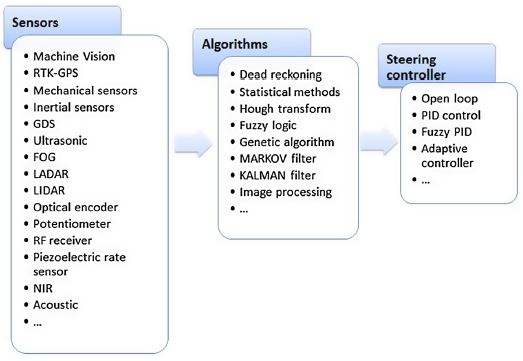
\includegraphics[width=3.5in]{control}
	\caption{Basic control diagram of autonomous vehicles.}
	\label{fig:con}
\end{figure}

In North America, the study “Agricultural automatic guidance research in North America” was published. It was established that Agricultural-related guidance research in North America has been review. Sensing Technologies were utilized and it was combined for automatic guidance. Automation depends on the ability of the researchers to maximize the performance of systems. Fig.~\ref{fig:elemen} shows the basic elements of agricultural vehicle automation systems.

\begin{figure}[!h]
	\centering
	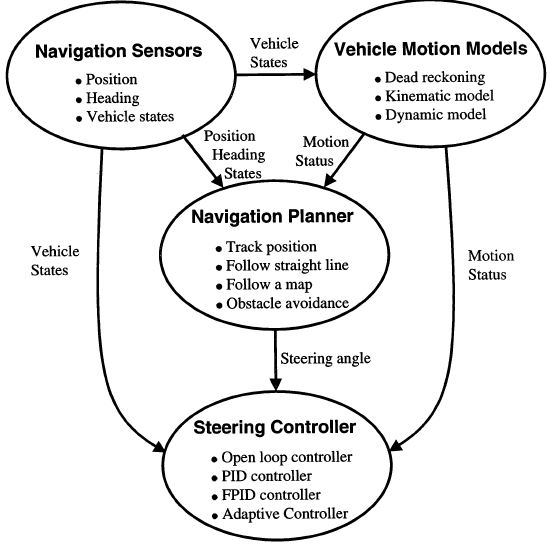
\includegraphics[width=3.5in]{elemen}
	\caption{Basic elements of agricultural vehicle automation systems}
	\label{fig:elemen}
\end{figure}

A similar study was implemented in Germany with the title “Automatic guidance for agricultural vehicles in Europe” was published. This paper focused on the automatic guidance of automatic agricultural vehicles. Different types of sensor and machine vision were used to implement the study. In line with the machine vision fragment, the row arrangement of crops were significantly considered in the development of the vehicle that utilizes machine vision. Fig.~\ref{fig:digit} shows the images related to the field tests performed. The image was digitized and guidelines were added.

\begin{figure}[!h]
	\centering
	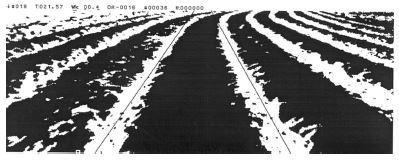
\includegraphics[width=3.5in]{digit}
	\caption{Digitised image with guidelines.}
	\label{fig:digit}
\end{figure}

One research is about the autonomous agriculture vehicles in Japan. This research has been developed in universities and government institutes, and by agricultural machinery manufacturers. The research wasn’t able to push through the whole research in the universities due to funding limitations, because of this research in universities has concentrated on methodologies, such as navigation, sensing, and application of control theory. Development of a one dimensional image sensor, and application of neural networks and genetic algorithms, has taken place at Hokkaido University; vision guidance and fuzzy logic application at the University of Tokyo; an automatic follow-up vehicle has been developed at Kyoto University; and an automatic transport vehicle at Ehime University. At research institutes and manufacturers, with their greater financial freedom, more practical systems have been developed. A tilling robot and a driver-less air blast sprayer is being developed in the Bio-oriented Technology Research Advancement Institute (BRAIN); and an autonomous rice planter, a tillage robot and autonomous forage tractor in the research institute of the Ministry of Agriculture, Forestry, and Fishery (MAFF). Kubota Co. Ltd has developed autonomous rice planting and husbandry vehicles. 

Another research is about the variable field-of-view machine vision based row guidance of agricultural robot. A new variable field-of-view machine vision method was developed allowing an agricultural robot to navigate between rows in cornfields. The machine vision hardware consisted of a camera with pitch and yaw motion control. Guidance lines were detected using an image-processing algorithm, employing morphological features in a far, near and lateral field of view, and the robot was guided along these lines using fuzzy logic control. The vehicle that they tested successfully traveled through a distance of 30 m towards the end of a crop row in three replications. 

Another article discusses the navigation system for agricultural machines. This article presents a new kind of navigation system for agricultural machines. The focus is on trajectory control where a Nonlinear Model Predictive path tracking for tractor and trailer system is presented. The experiments of the proposed method are carried out by using real agricultural machines in real environments. The goal of the research was to build a system, which is able to have at least the same accuracy as a human driver. The sufficient accuracy requirement was at most 10 cm lateral error at a speed of 12 km/h. The results presented in the article show that the goal was met and NMPC is a feasible method for accurate path tracking. 




\stopcontents[chapters]
\cleardoublepage


%%%%%%%%%%%%%%%%%%%%%%%%%%%%%%%%%%%%%%%%%%%%%%%%

%\chapter{Theoretical Considerations}
%\chaptermark{Theoretical Considerations} % uncomment this and put a shorter version of the chapter title for the TOC and chapter markings (i.e., header or footer)
%\label{ch:theorycon}
%\startcontents[chapters]
%\begin{SingleSpace}	
%	\Mprintcontents 
%\end{SingleSpace}
%\Blindtext

\begin{figure}[!htbp]
	\centering
		
\includegraphics[width=0.5\textwidth]{example}
	\caption{A quadrilateral image example.}
	\label{fig:exampletc}
\end{figure}

\section{Summary}
%\stopcontents[chapters]
%\cleardoublepage

%%%%%%%%%%%%%%%%%%%%%%%%%%%%%%%%%%%%%%%%%%%%%%%%
%\chapter{Design Considerations} 
%\label{ch:designcon} 
%\startcontents[chapters]
%\begin{SingleSpace}	
%	\Mprintcontents 
%\end{SingleSpace}
%\Blindtext

\section{Summary}
%\stopcontents[chapters]
%\cleardoublepage

%%%%%%%%%%%%%%%%%%%%%%%%%%%%%%%%%%%%%%%%%%%%%%%%
%\chapter{Methodology} 
%\label{ch:method} 
%\startcontents[chapters]
%\begin{SingleSpace}	
%	\Mprintcontents 
%\end{SingleSpace}
%\section{Implementation}

\Blindtext



\section{Evaluation}

\Blindtext



\section{Summary}

%\stopcontents[chapters]
%\cleardoublepage

%%%%%%%%%%%%%%%%%%%%%%%%%%%%%%%%%%%%%%%%%%%%%%%%
%\ifResultDiscuss 
%	\chapter{Results and Discussion} 
%	\label{ch:result_discuss} 
%	\startcontents[chapters]
%	\begin{SingleSpace}	
%		\Mprintcontents 
%	\end{SingleSpace}
%	\Blindtext

\section{Summary}
%	\stopcontents[chapters]
%	\cleardoublepage
%\fi

%%%%%%%%%%%%%%%%%%%%%%%%%%%%%%%%%%%%%%%%%%%%%%%%
%\ifConc
%	\chapter{Conclusions, Recommendations, and Future Directives} 
%	\label{ch:conc} 
%	\startcontents[chapters]
%	\begin{SingleSpace}	
%		\Mprintcontents 
%	\end{SingleSpace}
%	\section{Concluding Remarks}

In this \documentType, \ldots

\section{Contributions}

The interrelated \index{contributions} contributions and supplements that have been developed in this \documentType are listed as follows.

\begin{itemize}
  \item the ; 
	
	\item the ; 
  
  \item the ; 
	
\end{itemize}


\section{Recommendations}

\Blindtext

\section{Future Prospects}

There are several prospect related in this research that may be extended for further studies. \ldots So the suggested topics are listed in the following.

\begin{enumerate}
	\item  the \ldots.
	
	\item  the \ldots.
		
	\item  the \ldots.
\end{enumerate}



%	\stopcontents[chapters]
%	\cleardoublepage
%\fi

%%%%%%%%%%%%%%%%%%%%%%%%%%%%%%%%%%%%%%%%%%%%%%%
\renewcommand{\UrlFont}{\normalfont}
%\bibliographystyle{IEEEtr} % for IEEE referencing format
\bibliographystyle{apalike} % for APA referencing format
\begin{SingleSpace}
	{\small \bibliography{references}}
\end{SingleSpace}
\vfill
\begin{flushright}
Produced: \usdate\today, \currenttime \\
\end{flushright}
\cleardoublepage 

%%%%%%%%%%%%%%%%%%%%%%%%%%%%%%%%%%%%%%%%%%%%%%%%
\SingleSpacing
\appendix
\renewcommand{\thechapter}{\Alph{chapter}}
\renewcommand{\thesection}{\thechapter\arabic{section}}
\appto\appendix{\renewcommand\thechapter{\AlphAlph{\value{chapter}}}} % for increasing appendix chapters beyond Z, i.e. AA, AB, etc.
\chapter{Answers to Questions to this \documentType}
\startcontents[chapters]
\Mprintcontents 



\section{How important is the problem to practice?}

\blindtext
	
	
	
	
\section{How will you know if the solution/s that you will achieve would be better than existing ones?}	

\blindtext

\subsection{How will you measure the improvement/s?}	

\blindtext
	
\subsubsection{What is/are your basis/bases for the improvement/s?}

\blindtext
		
\subsubsection{Why did you choose that/those basis/bases?}

\blindtext
				
\subsubsection{How significant are your measure/s of the improvement/s?}

\blindtext






	
\section{What is the difference of the solution/s from existing ones?}
	
\blindtext

\subsection{How is it different from previous and existing ones?}

\blindtext
	
	
	
	
	
	
\section{What are the assumptions made (that are behind for your proposed solution to work)?}
	
\blindtext
		
	
\subsection{Will your proposed solution/s be sensitive to these assumptions?}
	
\blindtext

  
\subsection{Can your proposed solution/s be applied to more general cases when some of the assumptions are eliminated? If so, how?}

\blindtext






\section{What is the necessity of your approach / proposed solution/s?}

\blindtext
	
\subsection{What will be the limits of applicability of your proposed~solution/s?}

\blindtext
					  
\subsection{What will be the message of the proposed solution to technical people?  How about to non-technical managers and business men?}
			
\blindtext





\section{How will you know if your proposed solution/s is/are correct?}

\blindtext 
			
\subsection{Will your results warrant the level of mathematics used (i.e., will the end justify the means)?}
	    
\blindtext
			





\section{Is/are there an/\_ alternative way/s to get to the same solution/s?}

\blindtext
	
\subsection{Can you come up with illustrating examples, or even better, counter examples to your proposed solution/s?}

\blindtext
	
\subsection{Is there an approximation that can arrive at the essentially the same proposed solution/s more easily?}
	
\blindtext
			
	
	
	
	
\section{If you were the examiner of your proposal, how would you present the proposal in another way?}
	
\blindtext
	
	
\subsection{What are the weaknesses of your proposal?}

\blindtext

\stopcontents[chapters]
\cleardoublepage

%%%%%%%%%%%%%%%%%%%%%%%%%%%%%%%%%%%%%%%%%%%%%%%%
\chapter{Usage Examples} 
\label{ch:usage_examples}
% \startcontents[chapters]
% \Mprintcontents  
The user is expected to have a working knowledge of \LaTeX. A good introduction is in~\cite{Oetiker2014}.  Its latest version can be accessed at \url{http://www.ctan.org/tex-archive/info/lshort}.




\section{Equations}
\label{sec:eqn_not}

The following examples show how to typeset equations in \LaTeX.  This section also shows examples of the use of \verb| \gls{ } | commands in conjunction with the items that are in the \verb| notation.tex | file. \textbf{Please make sure that the entries in} \verb| notation.tex |\textbf{  are those that are referenced in the \LaTeX \ document files used by this \documentType.  Please comment out unused notations and be careful with the commas and brackets  in} \verb| notation.tex |.

In~\eqref{eq:conv}, the output signal \gls{not:output_sigt} is the result of the convolution of the input signal \gls{not:input_sigt} and the impulse response \gls{not:ir}.

\begin{eqnarray}   
     y\left( t \right) = h\left( t \right) * x\left( t \right)=\int_{-\infty}^{+\infty}h\left( t-\tau \right)x\left( \tau \right) \mathrm{d}\tau
	\label{eq:conv}
\end{eqnarray}

Other example equations are as follows.

\begin{eqnarray}
	\left[ \dfrac{ V_{1} }{ I_{1} } \right] = 
	\begin{bmatrix}
		A & B \\ 
		C & D 
	\end{bmatrix} 
	\left[ \dfrac{ V_{2} }{ I_{2} } \right]
	\label{eq:ABCD}
\end{eqnarray}

\begin{eqnarray}
\dfrac{1}{2} < \left\lfloor \mathrm{mod}\left(\left\lfloor \dfrac{y}{17} \right\rfloor 2^{-17 \lfloor x \rfloor - \mathrm{mod}(\lfloor y\rfloor, 17)},2\right)\right\rfloor,
\end{eqnarray}

\begin{eqnarray}
| \zeta(x)^3 \zeta(x + iy)^4 \zeta(x + 2iy) | = 
\exp\sum_{n,p} \frac{3 + 4 \cos( ny \log p) + \cos (2ny \log p)}{np^{nx}} \ge 1
\end{eqnarray}

\newpage
The verbatim \LaTeX \ code of Sec.~\ref{sec:eqn_not} is in List.~\ref{lst:eqn_gls}.

\begin{lstlisting}[
float=h,
caption=Sample \LaTeX \ code for equations and notations usage, 
label=lst:eqn_gls,
language=TeX,
frame=single]
The following examples show how to typeset equations in \LaTeX. 

In~\eqref{eq:conv}, the output signal \gls{not:output_sigt} is the result of the convolution of the input signal \gls{not:input_sigt} and the impulse response \gls{not:ir}.

\begin{eqnarray}   
     y\left( t \right) = h\left( t \right) * x\left( t \right)=\int_{-\infty}^{+\infty}h\left( t-\tau \right)x\left( \tau \right) \mathrm{d}\tau
	\label{eq:conv}
\end{eqnarray}

Other example equations are as follows.

\begin{eqnarray}
	\left[ \dfrac{ V_{1} }{ I_{1} } \right] = 
	\begin{bmatrix}
		A & B \\ 
		C & D 
	\end{bmatrix} 
	\left[ \dfrac{ V_{2} }{ I_{2} } \right]
	\label{eq:ABCD}
\end{eqnarray}

\begin{eqnarray}
{1\over 2} < \left\lfloor \mathrm{mod}\left(\left\lfloor {y \over 17} \right\rfloor 2^{-17 \lfloor x \rfloor - \mathrm{mod}(\lfloor y\rfloor, 17)},2\right)\right\rfloor,
\end{eqnarray}

\begin{eqnarray}
| \zeta(x)^3\zeta(x+iy)^4\zeta(x+2iy) | = 
\exp\sum_{n,p}\frac{3+4\cos(ny\log p) +\cos (2ny\log p)}{np^{nx}}\ge 1
\end{eqnarray}
\end{lstlisting}
\cleardoublepage







\newpage
\section{Notations}
\label{sec:not}
In order to use the standardized notation, the user is highly suggested to see the ISO~80000-2 standard~\cite{ISO800002}. The following were taken from \verb| isomath-test.tex |.

% A teststring with Latin and Greek letters::
\newcommand{\teststring}{%
% capital Latin letters
% A,B,C,
A,B,
% capital Greek letters
%\Gamma,\Delta,\Theta,\Lambda,\Xi,\Pi,\Sigma,\Upsilon,\Phi,\Psi,
\Gamma,\Delta,\Theta,\Lambda,\Xi,\Pi,\Sigma,\Phi,\Psi,\Omega,
% small Greek letters
\alpha,\beta,\pi,\nu,\omega,
% small Latin letters:
% compare \nu, \omega, v, and w
v,w,
% digits
0,1,9
}


\subsection*{Math alphabets}

If there are other symbols in place of Greek letters in a math
alphabet, it uses T1 or OT1 font encoding instead of OML.

\begin{eqnarray*}
\mbox{mathnormal} &  & \teststring \\
\mbox{mathit} &  & \mathit{\teststring}\\
\mbox{mathrm} &  & \mathrm{\teststring}\\
\mbox{mathbf} &  & \mathbf{\teststring}\\
\mbox{mathsf} &  & \mathsf{\teststring}\\
\mbox{mathtt} &  & \mathtt{\teststring}
\end{eqnarray*}
 New alphabets bold-italic, sans-serif-italic, and sans-serif-bold-italic.
\begin{eqnarray*}
\mbox{mathbfit}     &  & \mathbfit{\teststring}\\
\mbox{mathsfit}     &  & \mathsfit{\teststring}\\
\mbox{mathsfbfit} &  & \mathsfbfit{\teststring}
\end{eqnarray*}
%
Do the math alphabets match?

$
\mathnormal  {a x \alpha \omega}
\mathbfit    {a x \alpha \omega}
\mathsfbfit{a x \alpha \omega}
\quad
\mathsfbfit{T C \Theta \Gamma}
\mathbfit    {T C \Theta \Gamma}
\mathnormal  {T C \Theta \Gamma}
$

\subsection*{Vector symbols}

Alphabetic symbols for vectors are boldface italic,
$\vec{\lambda}=\vec{e}_{1}\cdot\vec{a}$,
while numeric ones (e.g. the zero vector) are bold upright,
$\vec{a} + \vec{0} = \vec{a}$.

\subsection*{Matrix symbols}

Symbols for matrices are boldface italic, too:%
\footnote{However, matrix symbols are usually capital letters whereas vectors
are small ones. Exceptions are physical quantities like the force
vector $\vec{F}$ or the electrical field $\vec{E}$.%
}
$\matrixsym{\Lambda}=\matrixsym{E}\cdot\matrixsym{A}.$


\subsection*{Tensor symbols}

Symbols for tensors are sans-serif bold italic,

\[
   \tensorsym{\alpha}  =  \tensorsym{e}\cdot\tensorsym{a}
   \quad \Longleftrightarrow \quad
   \alpha_{ijl}  =  e_{ijk}\cdot a_{kl}.
\]


The permittivity tensor describes the coupling of electric field and
displacement: \[
\vec{D}=\epsilon_{0}\tensorsym{\epsilon}_{\mathrm{r}}\vec{E}\]



\newpage
\subsection*{Bold math version}

The ``bold'' math version is selected with the commands
\verb+\boldmath+ or \verb+\mathversion{bold}+

{\boldmath
	\begin{eqnarray*}
	\mbox{mathnormal} &  & \teststring \\
	\mbox{mathit} &  & \mathit{\teststring}\\
	\mbox{mathrm} &  & \mathrm{\teststring}\\
	\mbox{mathbf} &  & \mathbf{\teststring}\\
	\mbox{mathsf} &  & \mathsf{\teststring}\\
	\mbox{mathtt} &  & \mathtt{\teststring}
	\end{eqnarray*}
	 New alphabets bold-italic, sans-serif-italic, and sans-serif-bold-italic.
	\begin{eqnarray*}
	\mbox{mathbfit}     &  & \mathbfit{\teststring}\\
	\mbox{mathsfit}     &  & \mathsfit{\teststring}\\
	\mbox{mathsfbfit} &  & \mathsfbfit{\teststring}
	\end{eqnarray*}
	%
	Do the math alphabets match?

	$
	\mathnormal  {a x \alpha \omega}
	\mathbfit    {a x \alpha \omega}
	\mathsfbfit{a x \alpha \omega}
	\quad
	\mathsfbfit{T C \Theta \Gamma}
	\mathbfit    {T C \Theta \Gamma}
	\mathnormal  {T C \Theta \Gamma}
	$

	\subsection*{Vector symbols}

	Alphabetic symbols for vectors are boldface italic,
	$\vec{\lambda}=\vec{e}_{1}\cdot\vec{a}$,
	while numeric ones (e.g. the zero vector) are bold upright,
	$\vec{a} + \vec{0} = \vec{a}$.




	\subsection*{Matrix symbols}

	Symbols for matrices are boldface italic, too:%
	\footnote{However, matrix symbols are usually capital letters whereas vectors
	are small ones. Exceptions are physical quantities like the force
	vector $\vec{F}$ or the electrical field $\vec{E}$.%
	}
	$\matrixsym{\Lambda}=\matrixsym{E}\cdot\matrixsym{A}.$


	\subsection*{Tensor symbols}

	Symbols for tensors are sans-serif bold italic,

	\[
		 \tensorsym{\alpha}  =  \tensorsym{e}\cdot\tensorsym{a}
		 \quad \Longleftrightarrow \quad
		 \alpha_{ijl}  =  e_{ijk}\cdot a_{kl}.
	\]

	The permittivity tensor describes the coupling of electric field and
	displacement: \[
	\vec{D}=\epsilon_{0}\tensorsym{\epsilon}_{\mathrm{r}}\vec{E}\]
}











\newpage
The verbatim \LaTeX \ code of Sec.~\ref{sec:not} is in List.~\ref{lst:not}.

\begin{lstlisting}[
%float=h,% do not use float option for long listings
caption=Sample \LaTeX \ code for notations usage, 
label=lst:not,
language=TeX,
frame=single]
% A teststring with Latin and Greek letters::
\newcommand{\teststring}{%
% capital Latin letters
% A,B,C,
A,B,
% capital Greek letters
%\Gamma,\Delta,\Theta,\Lambda,\Xi,\Pi,\Sigma,\Upsilon,\Phi,\Psi,
\Gamma,\Delta,\Theta,\Lambda,\Xi,\Pi,\Sigma,\Phi,\Psi,\Omega,
% small Greek letters
\alpha,\beta,\pi,\nu,\omega,
% small Latin letters:
% compare \nu, \omega, v, and w
v,w,
% digits
0,1,9
}


\subsection*{Math alphabets}

If there are other symbols in place of Greek letters in a math
alphabet, it uses T1 or OT1 font encoding instead of OML.

\begin{eqnarray*}
\mbox{mathnormal} &  & \teststring \\
\mbox{mathit} &  & \mathit{\teststring}\\
\mbox{mathrm} &  & \mathrm{\teststring}\\
\mbox{mathbf} &  & \mathbf{\teststring}\\
\mbox{mathsf} &  & \mathsf{\teststring}\\
\mbox{mathtt} &  & \mathtt{\teststring}
\end{eqnarray*}
 New alphabets bold-italic, sans-serif-italic, and sans-serif-bold-italic.
\begin{eqnarray*}
\mbox{mathbfit}     &  & \mathbfit{\teststring}\\
\mbox{mathsfit}     &  & \mathsfit{\teststring}\\
\mbox{mathsfbfit} &  & \mathsfbfit{\teststring}
\end{eqnarray*}
%
Do the math alphabets match?

$
\mathnormal  {a x \alpha \omega}
\mathbfit    {a x \alpha \omega}
\mathsfbfit{a x \alpha \omega}
\quad
\mathsfbfit{T C \Theta \Gamma}
\mathbfit    {T C \Theta \Gamma}
\mathnormal  {T C \Theta \Gamma}
$

\subsection*{Vector symbols}

Alphabetic symbols for vectors are boldface italic,
$\vec{\lambda}=\vec{e}_{1}\cdot\vec{a}$,
while numeric ones (e.g. the zero vector) are bold upright,
$\vec{a} + \vec{0} = \vec{a}$.

\subsection*{Matrix symbols}

Symbols for matrices are boldface italic, too:%
\footnote{However, matrix symbols are usually capital letters whereas vectors
are small ones. Exceptions are physical quantities like the force
vector $\vec{F}$ or the electrical field $\vec{E}$.%
}
$\matrixsym{\Lambda}=\matrixsym{E}\cdot\matrixsym{A}.$


\subsection*{Tensor symbols}

Symbols for tensors are sans-serif bold italic,

\[
   \tensorsym{\alpha}  =  \tensorsym{e}\cdot\tensorsym{a}
   \quad \Longleftrightarrow \quad
   \alpha_{ijl}  =  e_{ijk}\cdot a_{kl}.
\]


The permittivity tensor describes the coupling of electric field and
displacement: \[
\vec{D}=\epsilon_{0}\tensorsym{\epsilon}_{\mathrm{r}}\vec{E}\]



\newpage
\subsection*{Bold math version}

The ``bold'' math version is selected with the commands
\verb+\boldmath+ or \verb+\mathversion{bold}+

{\boldmath
	\begin{eqnarray*}
	\mbox{mathnormal} &  & \teststring \\
	\mbox{mathit} &  & \mathit{\teststring}\\
	\mbox{mathrm} &  & \mathrm{\teststring}\\
	\mbox{mathbf} &  & \mathbf{\teststring}\\
	\mbox{mathsf} &  & \mathsf{\teststring}\\
	\mbox{mathtt} &  & \mathtt{\teststring}
	\end{eqnarray*}
	 New alphabets bold-italic, sans-serif-italic, and sans-serif-bold-italic.
	\begin{eqnarray*}
	\mbox{mathbfit}     &  & \mathbfit{\teststring}\\
	\mbox{mathsfit}     &  & \mathsfit{\teststring}\\
	\mbox{mathsfbfit} &  & \mathsfbfit{\teststring}
	\end{eqnarray*}
	%
	Do the math alphabets match?

	$
	\mathnormal  {a x \alpha \omega}
	\mathbfit    {a x \alpha \omega}
	\mathsfbfit{a x \alpha \omega}
	\quad
	\mathsfbfit{T C \Theta \Gamma}
	\mathbfit    {T C \Theta \Gamma}
	\mathnormal  {T C \Theta \Gamma}
	$

	\subsection*{Vector symbols}

	Alphabetic symbols for vectors are boldface italic,
	$\vec{\lambda}=\vec{e}_{1}\cdot\vec{a}$,
	while numeric ones (e.g. the zero vector) are bold upright,
	$\vec{a} + \vec{0} = \vec{a}$.




	\subsection*{Matrix symbols}

	Symbols for matrices are boldface italic, too:%
	\footnote{However, matrix symbols are usually capital letters whereas vectors
	are small ones. Exceptions are physical quantities like the force
	vector $\vec{F}$ or the electrical field $\vec{E}$.%
	}
	$\matrixsym{\Lambda}=\matrixsym{E}\cdot\matrixsym{A}.$


	\subsection*{Tensor symbols}

	Symbols for tensors are sans-serif bold italic,

	\[
		 \tensorsym{\alpha}  =  \tensorsym{e}\cdot\tensorsym{a}
		 \quad \Longleftrightarrow \quad
		 \alpha_{ijl}  =  e_{ijk}\cdot a_{kl}.
	\]

	The permittivity tensor describes the coupling of electric field and
	displacement: \[
	\vec{D}=\epsilon_{0}\tensorsym{\epsilon}_{\mathrm{r}}\vec{E}\]
}

\end{lstlisting}
\cleardoublepage











\newpage
\section{Abbreviation}\
\label{sec:abbrv}

This section shows examples of the use of \LaTeX commands in conjunction with the items that are in the \verb| abbreviation.tex | and in the \verb| glossary.tex | files.  Please see List.~\ref{lst:abbrv}. \textbf{To lessen the \LaTeX \ compilation time, it is suggested that you use} \verb| \acr{ } | \textbf{only for the first occurrence of the word to be abbreviated.}

Again please see List.~\ref{lst:abbrv}. Here is an example of first use: \acr{ac}. Next use: \acr{ac}. Full: \gls{ac}.  Here's an acronym referenced using \verb| \acr |: \acr{html}.  And here it is again: \acr{html}. If you are used to the \texttt{glossaries} package, note the difference in using \verb| \gls |: \gls{html}. And again (no difference): \gls{html}. Here are some more entries:

\begin{itemize}

	\item \acr{xml} and \acr{css}.

	\item Next use: \acr{xml} and \acr{css}.

	\item Full form: \gls{xml} and \gls{css}.

	\item Reset again. \glsresetall{abbreviation}

	\item Start with a capital. \Acr{html}.

	\item Next: \Acr{html}. Full: \Gls{html}.

	\item Prefer capitals? \renewcommand{\acronymfont}[1]{\MakeTextUppercase{#1}} \Acr{xml}. Next: \acr{xml}. Full: \gls{xml}.

	\item Prefer small-caps? \renewcommand{\acronymfont}[1]{\textsc{#1}} \Acr{css}. Next: \acr{css}. Full: \gls{css}.

	\item Resetting all acronyms.\glsresetall{abbreviation}

	\item Here are the acronyms again:

	\item \Acr{html}, \acr{xml} and \acr{css}.

	\item Next use: \Acr{html}, \acr{xml} and \acr{css}.

	\item Full form: \Gls{html}, \gls{xml} and \gls{css}.

	\item Provide your own link text: \glslink{[textbf]css}{style sheet}.

\end{itemize}



The verbatim \LaTeX \ code of Sec.~\ref{sec:abbrv} is in List.~\ref{lst:abbrv}.

\begin{lstlisting}[
float=h,
caption=Sample \LaTeX \ code for abbreviations usage, 
label=lst:abbrv,
language=TeX,
frame=single]
Again please see List.~\ref{lst:abbrv}. Here is an example of first use: \acr{ac}. Next use: \acr{ac}. Full: \gls{ac}.  Here's an acronym referenced using \verb| \acr |: \acr{html}.  And here it is again: \acr{html}. If you are used to the \texttt{glossaries} package, note the difference in using \verb| \gls |: \gls{html}. And again (no difference): \gls{html}. Here are some more entries:

\begin{itemize}

	\item \acr{xml} and \acr{css}.

	\item Next use: \acr{xml} and \acr{css}.

	\item Full form: \gls{xml} and \gls{css}.

	\item Reset again. \glsresetall{abbreviation}

	\item Start with a capital. \Acr{html}.

	\item Next: \Acr{html}. Full: \Gls{html}.

	\item Prefer capitals? \renewcommand{\acronymfont}[1]{\MakeTextUppercase{#1}} \Acr{xml}. Next: \acr{xml}. Full: \gls{xml}.

	\item Prefer small-caps? \renewcommand{\acronymfont}[1]{\textsc{#1}} \Acr{css}. Next: \acr{css}. Full: \gls{css}.

	\item Resetting all acronyms.\glsresetall{abbreviation}

	\item Here are the acronyms again:

	\item \Acr{html}, \acr{xml} and \acr{css}.

	\item Next use: \Acr{html}, \acr{xml} and \acr{css}.

	\item Full form: \Gls{html}, \gls{xml} and \gls{css}.

	\item Provide your own link text: \glslink{[textbf]css}{style} 
	
\end{itemize}
\end{lstlisting}
\cleardoublepage






\newpage
\section{Glossary}
\label{sec:glos}

This section shows examples of the use of \verb| \gls{ } | commands in conjunction with the items that are in the \verb| glossary.tex | and \verb| notation.tex | files.  Note that entries in  \verb| notation.tex |  are prefixed with ``\verb| not: |'' label (see List.~\ref{lst:glos}).

\textbf{Please make sure that the entries in} \verb| notation.tex |\textbf{  are those that are referenced in the \LaTeX \ document files used by this \documentType.  Please comment out unused notations and be careful with the commas and brackets  in} \verb| notation.tex |.

\begin{itemize}

	\item \Glspl{matrix} are usually denoted by a bold capital letter, such as $\mathbfit{A}$. The \gls{matrix}'s $(i,j)$th element is usually denoted $a_{ij}$. \Gls{matrix} $\mathbf{I}$ is the identity \gls{matrix}.

	\item A set, denoted as \gls{not:set}, is a collection of objects.

	\item The universal set,  denoted as \gls{not:universalSet}, is the set of everything.

	\item The empty set, denoted as \gls{not:emptySet}, contains no elements.

	\item The cardinality of a set, denoted as \gls{not:cardinality}, is the number of elements in the set.

\end{itemize}


The verbatim \LaTeX \ code for the part of Sec.~\ref{sec:glos} is in List.~\ref{lst:glos}.

\begin{lstlisting}[
float=h,
caption=Sample \LaTeX \ code for glossary and notations usage, 
label=lst:glos,
language=TeX,
frame=single]
\begin{itemize}

	\item \Glspl{matrix} are usually denoted by a bold capital letter, such as $\mathbfit{A}$. The \gls{matrix}'s $(i,j)$th element is usually denoted $a_{ij}$. \Gls{matrix} $\mathbf{I}$ is the identity \gls{matrix}.

	\item A set, denoted as \gls{not:set}, is a collection of objects.

	\item The universal set,  denoted as \gls{not:universalSet}, is the set of everything.

	\item The empty set, denoted as \gls{not:emptySet}, contains no elements.

	\item The cardinality of a set, denoted as \gls{not:cardinality}, is the number of elements in the set.

\end{enumerate}
\end{lstlisting}
\cleardoublepage












\newpage
\section{Figure}

This section shows several ways of placing figures.  PDF\LaTeX \ compatible files are PDF, PNG, and JPG.  Please see the \verb| figure | subdirectory.

\begin{figure}[!htbp]
	\centering
		
\includegraphics[width=0.5\textwidth]{example}
	\caption{A quadrilateral image example.}
	\label{fig:example}
\end{figure}
\cleardoublepage

Fig.~\ref{fig:example} is a gray box enclosed by a dark border. List.~\ref{lst:onefig} shows the corresponding \LaTeX \ code. 


\begin{lstlisting}[
float=h,
caption=Sample \LaTeX \ code for a single figure, 
label=lst:onefig,
language=TeX,
frame=single]
\begin{figure}[!htbp]
	\centering
		
\includegraphics[width=0.5\textwidth]{example}
	\caption{A quadrilateral image example.}
	\label{fig:example}
\end{figure}
\cleardoublepage

Fig.~\ref{fig:example} is a gray box enclosed by a dark border. List.~\ref{lst:onefig} shows the corresponding \LaTeX \ code. 	
\end{figure}
\end{lstlisting}
\cleardoublepage





\begin{figure}[!htbp]
\centering
\subbottom[A sub-figure in the top row.]{

\includegraphics[width=0.35\textwidth]{example}
\label{fig:top}
}
\vfill
\subbottom[A sub-figure in the middle row.]{

\includegraphics[width=0.35\textwidth]{example}
\label{fig:mid}
}
\vfill
\subbottom[A sub-figure in the bottom row.]{

\includegraphics[width=0.35\textwidth]{example}
\label{fig:botm}
}
\caption{Figures on top of each other. See List.~\ref{lst:figsontop} for the corresponding \LaTeX \ code. } 
\label{fig:tmb}
\end{figure}
\cleardoublepage




\begin{lstlisting}[
float=h,
caption=Sample \LaTeX \ code for three figures on top of each other, 
label=lst:figsontop,
language=TeX,
frame=single]
\begin{figure}[!htbp]
\centering
\subbottom[A sub-figure in the top row.]{

\includegraphics[width=0.35\textwidth]{example}
\label{fig:top}
}
\vfill
\subbottom[A sub-figure in the middle row.]{

\includegraphics[width=0.35\textwidth]{example}
\label{fig:mid}
}
\vfill
\subbottom[A sub-figure in the bottom row.]{

\includegraphics[width=0.35\textwidth]{example}
\label{fig:botm}
}
\caption{Figures on top of each other} 
\label{fig:tmb}
\end{figure}
\end{lstlisting}
\cleardoublepage







\begin{figure}[!htbp]
\centering
\subbottom[A sub-figure in the upper-left corner.]{

\includegraphics[width=0.45\textwidth]{example}
\label{fig:upprleft}
}
\hfill
\subbottom[A sub-figure in the upper-right corner.]{

\includegraphics[width=0.45\textwidth]{example}
\label{fig:uppright}
}
\vfill
\subbottom[A sub-figure in the lower-left corner.]{

\includegraphics[width=0.45\textwidth]{example}
\label{fig:lowerleft}
}
\hfill
\subbottom[A sub-figure in the lower-right corner]{

\includegraphics[width=0.45\textwidth]{example}
\label{fig:lowright}
}
\caption{Four figures in each corner. See List.~\ref{lst:fourfigs} for the corresponding \LaTeX \ code.} 
\label{fig:fourfig}
\end{figure}
\cleardoublepage




\begin{lstlisting}[
float=h,
caption=Sample \LaTeX \ code for the four figures, 
label=lst:fourfigs,
language=TeX,
frame=single]
\begin{figure}[!htbp]
\centering
\subbottom[A sub-figure in the upper-left corner.]{

\includegraphics[width=0.45\textwidth]{example}
\label{fig:upprleft}
}
\hfill
\subbottom[A sub-figure in the upper-right corner.]{

\includegraphics[width=0.45\textwidth]{example}
\label{fig:uppright}
}
\vfill
\subbottom[A sub-figure in the lower-left corner.]{

\includegraphics[width=0.45\textwidth]{example}
\label{fig:lowerleft}
}
\hfill
\subbottom[A sub-figure in the lower-right corner]{

\includegraphics[width=0.45\textwidth]{example}
\label{fig:lowright}
}
\caption{Four figures in each corner. See List.~\ref{lst:fourfigs} for the corresponding \LaTeX \ code.} 
\label{fig:fourfig}
\end{figure}
\end{lstlisting}
\cleardoublepage





\newpage
\section{Table}

This section shows an example of placing a table (a long one). Table~\ref{tab:triple_grid} are the triples. 

\begin{center}
{\scriptsize
\begin{tabularx}{\textwidth}{p{0.1\textwidth}|p{0.2\textwidth}|p{0.5\textwidth}}
\caption{Feasible triples for highly variable grid} \label{tab:triple_grid} \\
\hline 
\hline 
\textbf{Time (s)} & 
\textbf{Triple chosen} & 
\textbf{Other feasible triples} \\ 
\hline 
\endfirsthead
\multicolumn{3}{c}%
{\textit{Continued from previous page}} \\
\hline
\hline 
\textbf{Time (s)} & 
\textbf{Triple chosen} & 
\textbf{Other feasible triples} \\ 
\hline 
\endhead
\hline 
\multicolumn{3}{r}{\textit{Continued on next page}} \\ 
\endfoot
\hline 
\endlastfoot
\hline

0 & (1, 11, 13725) & (1, 12, 10980), (1, 13, 8235), (2, 2, 0), (3, 1, 0) \\
2745 & (1, 12, 10980) & (1, 13, 8235), (2, 2, 0), (2, 3, 0), (3, 1, 0) \\
5490 & (1, 12, 13725) & (2, 2, 2745), (2, 3, 0), (3, 1, 0) \\
8235 & (1, 12, 16470) & (1, 13, 13725), (2, 2, 2745), (2, 3, 0), (3, 1, 0) \\
10980 & (1, 12, 16470) & (1, 13, 13725), (2, 2, 2745), (2, 3, 0), (3, 1, 0) \\
13725 & (1, 12, 16470) & (1, 13, 13725), (2, 2, 2745), (2, 3, 0), (3, 1, 0) \\
16470 & (1, 13, 16470) & (2, 2, 2745), (2, 3, 0), (3, 1, 0) \\
19215 & (1, 12, 16470) & (1, 13, 13725), (2, 2, 2745), (2, 3, 0), (3, 1, 0) \\
21960 & (1, 12, 16470) & (1, 13, 13725), (2, 2, 2745), (2, 3, 0), (3, 1, 0) \\
24705 & (1, 12, 16470) & (1, 13, 13725), (2, 2, 2745), (2, 3, 0), (3, 1, 0) \\
27450 & (1, 12, 16470) & (1, 13, 13725), (2, 2, 2745), (2, 3, 0), (3, 1, 0) \\
30195 & (2, 2, 2745) & (2, 3, 0), (3, 1, 0) \\
32940 & (1, 13, 16470) & (2, 2, 2745), (2, 3, 0), (3, 1, 0) \\
35685 & (1, 13, 13725) & (2, 2, 2745), (2, 3, 0), (3, 1, 0) \\
38430 & (1, 13, 10980) & (2, 2, 2745), (2, 3, 0), (3, 1, 0) \\
41175 & (1, 12, 13725) & (1, 13, 10980), (2, 2, 2745), (2, 3, 0), (3, 1, 0) \\
43920 & (1, 13, 10980) & (2, 2, 2745), (2, 3, 0), (3, 1, 0) \\
46665 & (2, 2, 2745) & (2, 3, 0), (3, 1, 0) \\
49410 & (2, 2, 2745) & (2, 3, 0), (3, 1, 0) \\
52155 & (1, 12, 16470) & (1, 13, 13725), (2, 2, 2745), (2, 3, 0), (3, 1, 0) \\
54900 & (1, 13, 13725) & (2, 2, 2745), (2, 3, 0), (3, 1, 0) \\
57645 & (1, 13, 13725) & (2, 2, 2745), (2, 3, 0), (3, 1, 0) \\
60390 & (1, 12, 13725) & (2, 2, 2745), (2, 3, 0), (3, 1, 0) \\
63135 & (1, 13, 16470) & (2, 2, 2745), (2, 3, 0), (3, 1, 0) \\
65880 & (1, 13, 16470) & (2, 2, 2745), (2, 3, 0), (3, 1, 0) \\
68625 & (2, 2, 2745) & (2, 3, 0), (3, 1, 0) \\
71370 & (1, 13, 13725) & (2, 2, 2745), (2, 3, 0), (3, 1, 0) \\
74115 & (1, 12, 13725) & (2, 2, 2745), (2, 3, 0), (3, 1, 0) \\
76860 & (1, 13, 13725) & (2, 2, 2745), (2, 3, 0), (3, 1, 0) \\
79605 & (1, 13, 13725) & (2, 2, 2745), (2, 3, 0), (3, 1, 0) \\
82350 & (1, 12, 13725) & (2, 2, 2745), (2, 3, 0), (3, 1, 0) \\
85095 & (1, 12, 13725) & (1, 13, 10980), (2, 2, 2745), (2, 3, 0), (3, 1, 0) \\
87840 & (1, 13, 16470) & (2, 2, 2745), (2, 3, 0), (3, 1, 0) \\
90585 & (1, 13, 16470) & (2, 2, 2745), (2, 3, 0), (3, 1, 0) \\
93330 & (1, 13, 13725) & (2, 2, 2745), (2, 3, 0), (3, 1, 0) \\
96075 & (1, 13, 16470) & (2, 2, 2745), (2, 3, 0), (3, 1, 0) \\
98820 & (1, 13, 16470) & (2, 2, 2745), (2, 3, 0), (3, 1, 0) \\
101565 & (1, 13, 13725) & (2, 2, 2745), (2, 3, 0), (3, 1, 0) \\
104310 & (1, 13, 16470) & (2, 2, 2745), (2, 3, 0), (3, 1, 0) \\
107055 & (1, 13, 13725) & (2, 2, 2745), (2, 3, 0), (3, 1, 0) \\
109800 & (1, 13, 13725) & (2, 2, 2745), (2, 3, 0), (3, 1, 0) \\
112545 & (1, 12, 16470) & (1, 13, 13725), (2, 2, 2745), (2, 3, 0), (3, 1, 0) \\
115290 & (1, 13, 16470) & (2, 2, 2745), (2, 3, 0), (3, 1, 0) \\
118035 & (1, 13, 13725) & (2, 2, 2745), (2, 3, 0), (3, 1, 0) \\
120780 & (1, 13, 16470) & (2, 2, 2745), (2, 3, 0), (3, 1, 0) \\
123525 & (1, 13, 13725) & (2, 2, 2745), (2, 3, 0), (3, 1, 0) \\
126270 & (1, 12, 16470) & (1, 13, 13725), (2, 2, 2745), (2, 3, 0), (3, 1, 0) \\
129015 & (2, 2, 2745) & (2, 3, 0), (3, 1, 0) \\
131760 & (2, 2, 2745) & (2, 3, 0), (3, 1, 0) \\
134505 & (1, 13, 16470) & (2, 2, 2745), (2, 3, 0), (3, 1, 0) \\
137250 & (1, 13, 13725) & (2, 2, 2745), (2, 3, 0), (3, 1, 0) \\
139995 & (2, 2, 2745) & (2, 3, 0), (3, 1, 0) \\
142740 & (2, 2, 2745) & (2, 3, 0), (3, 1, 0) \\
145485 & (1, 12, 16470) & (1, 13, 13725), (2, 2, 2745), (2, 3, 0), (3, 1, 0) \\
148230 & (2, 2, 2745) & (2, 3, 0), (3, 1, 0) \\
150975 & (1, 13, 16470) & (2, 2, 2745), (2, 3, 0), (3, 1, 0) \\
153720 & (1, 12, 13725) & (2, 2, 2745), (2, 3, 0), (3, 1, 0) \\
156465 & (1, 13, 13725) & (2, 2, 2745), (2, 3, 0), (3, 1, 0) \\
159210 & (1, 13, 13725) & (2, 2, 2745), (2, 3, 0), (3, 1, 0) \\
161955 & (1, 13, 16470) & (2, 2, 2745), (2, 3, 0), (3, 1, 0) \\
164700 & (1, 13, 13725) & (2, 2, 2745), (2, 3, 0), (3, 1, 0) \\
\end{tabularx}
}
\end{center}
\cleardoublepage









List.~\ref{lst:tabl} shows the corresponding \LaTeX \ code. 

\begin{lstlisting}[
%float=h,% do not use float option for long listings
caption=Sample \LaTeX \ code for making typical table environment, 
label=lst:tabl,
language=TeX,
frame=single,]
\begin{center}
{\scriptsize
\begin{tabularx}{\textwidth}{p{0.1\textwidth}|p{0.2\textwidth}|p{0.5\textwidth}}
\caption{Feasible triples for highly variable grid} \label{tab:triple_grid} \\
\hline 
\hline 
\textbf{Time (s)} & 
\textbf{Triple chosen} & 
\textbf{Other feasible triples} \\ 
\hline 
\endfirsthead
\multicolumn{3}{c}%
{\textit{Continued from previous page}} \\
\hline
\hline 
\textbf{Time (s)} & 
\textbf{Triple chosen} & 
\textbf{Other feasible triples} \\ 
\hline 
\endhead
\hline 
\multicolumn{3}{r}{\textit{Continued on next page}} \\ 
\endfoot
\hline 
\endlastfoot
\hline

0 & (1, 11, 13725) & (1, 12, 10980), (1, 13, 8235), (2, 2, 0), (3, 1, 0) \\
2745 & (1, 12, 10980) & (1, 13, 8235), (2, 2, 0), (2, 3, 0), (3, 1, 0) \\
5490 & (1, 12, 13725) & (2, 2, 2745), (2, 3, 0), (3, 1, 0) \\
8235 & (1, 12, 16470) & (1, 13, 13725), (2, 2, 2745), (2, 3, 0), (3, 1, 0) \\
10980 & (1, 12, 16470) & (1, 13, 13725), (2, 2, 2745), (2, 3, 0), (3, 1, 0) \\
13725 & (1, 12, 16470) & (1, 13, 13725), (2, 2, 2745), (2, 3, 0), (3, 1, 0) \\
16470 & (1, 13, 16470) & (2, 2, 2745), (2, 3, 0), (3, 1, 0) \\
19215 & (1, 12, 16470) & (1, 13, 13725), (2, 2, 2745), (2, 3, 0), (3, 1, 0) \\
21960 & (1, 12, 16470) & (1, 13, 13725), (2, 2, 2745), (2, 3, 0), (3, 1, 0) \\
24705 & (1, 12, 16470) & (1, 13, 13725), (2, 2, 2745), (2, 3, 0), (3, 1, 0) \\
27450 & (1, 12, 16470) & (1, 13, 13725), (2, 2, 2745), (2, 3, 0), (3, 1, 0) \\
30195 & (2, 2, 2745) & (2, 3, 0), (3, 1, 0) \\
32940 & (1, 13, 16470) & (2, 2, 2745), (2, 3, 0), (3, 1, 0) \\
35685 & (1, 13, 13725) & (2, 2, 2745), (2, 3, 0), (3, 1, 0) \\
38430 & (1, 13, 10980) & (2, 2, 2745), (2, 3, 0), (3, 1, 0) \\
41175 & (1, 12, 13725) & (1, 13, 10980), (2, 2, 2745), (2, 3, 0), (3, 1, 0) \\
43920 & (1, 13, 10980) & (2, 2, 2745), (2, 3, 0), (3, 1, 0) \\
46665 & (2, 2, 2745) & (2, 3, 0), (3, 1, 0) \\
49410 & (2, 2, 2745) & (2, 3, 0), (3, 1, 0) \\
52155 & (1, 12, 16470) & (1, 13, 13725), (2, 2, 2745), (2, 3, 0), (3, 1, 0) \\
54900 & (1, 13, 13725) & (2, 2, 2745), (2, 3, 0), (3, 1, 0) \\
57645 & (1, 13, 13725) & (2, 2, 2745), (2, 3, 0), (3, 1, 0) \\
60390 & (1, 12, 13725) & (2, 2, 2745), (2, 3, 0), (3, 1, 0) \\
63135 & (1, 13, 16470) & (2, 2, 2745), (2, 3, 0), (3, 1, 0) \\
65880 & (1, 13, 16470) & (2, 2, 2745), (2, 3, 0), (3, 1, 0) \\
68625 & (2, 2, 2745) & (2, 3, 0), (3, 1, 0) \\
71370 & (1, 13, 13725) & (2, 2, 2745), (2, 3, 0), (3, 1, 0) \\
74115 & (1, 12, 13725) & (2, 2, 2745), (2, 3, 0), (3, 1, 0) \\
76860 & (1, 13, 13725) & (2, 2, 2745), (2, 3, 0), (3, 1, 0) \\
79605 & (1, 13, 13725) & (2, 2, 2745), (2, 3, 0), (3, 1, 0) \\
82350 & (1, 12, 13725) & (2, 2, 2745), (2, 3, 0), (3, 1, 0) \\
85095 & (1, 12, 13725) & (1, 13, 10980), (2, 2, 2745), (2, 3, 0), (3, 1, 0) \\
87840 & (1, 13, 16470) & (2, 2, 2745), (2, 3, 0), (3, 1, 0) \\
90585 & (1, 13, 16470) & (2, 2, 2745), (2, 3, 0), (3, 1, 0) \\
93330 & (1, 13, 13725) & (2, 2, 2745), (2, 3, 0), (3, 1, 0) \\
96075 & (1, 13, 16470) & (2, 2, 2745), (2, 3, 0), (3, 1, 0) \\
98820 & (1, 13, 16470) & (2, 2, 2745), (2, 3, 0), (3, 1, 0) \\
101565 & (1, 13, 13725) & (2, 2, 2745), (2, 3, 0), (3, 1, 0) \\
104310 & (1, 13, 16470) & (2, 2, 2745), (2, 3, 0), (3, 1, 0) \\
107055 & (1, 13, 13725) & (2, 2, 2745), (2, 3, 0), (3, 1, 0) \\
109800 & (1, 13, 13725) & (2, 2, 2745), (2, 3, 0), (3, 1, 0) \\
112545 & (1, 12, 16470) & (1, 13, 13725), (2, 2, 2745), (2, 3, 0), (3, 1, 0) \\
115290 & (1, 13, 16470) & (2, 2, 2745), (2, 3, 0), (3, 1, 0) \\
118035 & (1, 13, 13725) & (2, 2, 2745), (2, 3, 0), (3, 1, 0) \\
120780 & (1, 13, 16470) & (2, 2, 2745), (2, 3, 0), (3, 1, 0) \\
123525 & (1, 13, 13725) & (2, 2, 2745), (2, 3, 0), (3, 1, 0) \\
126270 & (1, 12, 16470) & (1, 13, 13725), (2, 2, 2745), (2, 3, 0), (3, 1, 0) \\
129015 & (2, 2, 2745) & (2, 3, 0), (3, 1, 0) \\
131760 & (2, 2, 2745) & (2, 3, 0), (3, 1, 0) \\
134505 & (1, 13, 16470) & (2, 2, 2745), (2, 3, 0), (3, 1, 0) \\
137250 & (1, 13, 13725) & (2, 2, 2745), (2, 3, 0), (3, 1, 0) \\
139995 & (2, 2, 2745) & (2, 3, 0), (3, 1, 0) \\
142740 & (2, 2, 2745) & (2, 3, 0), (3, 1, 0) \\
145485 & (1, 12, 16470) & (1, 13, 13725), (2, 2, 2745), (2, 3, 0), (3, 1, 0) \\
148230 & (2, 2, 2745) & (2, 3, 0), (3, 1, 0) \\
150975 & (1, 13, 16470) & (2, 2, 2745), (2, 3, 0), (3, 1, 0) \\
153720 & (1, 12, 13725) & (2, 2, 2745), (2, 3, 0), (3, 1, 0) \\
156465 & (1, 13, 13725) & (2, 2, 2745), (2, 3, 0), (3, 1, 0) \\
159210 & (1, 13, 13725) & (2, 2, 2745), (2, 3, 0), (3, 1, 0) \\
161955 & (1, 13, 16470) & (2, 2, 2745), (2, 3, 0), (3, 1, 0) \\
164700 & (1, 13, 13725) & (2, 2, 2745), (2, 3, 0), (3, 1, 0) \\
\end{tabularx}
}
\end{center} 
\end{lstlisting}
\cleardoublepage








\newpage
\section{Algorithm or Pseudocode Listing}

Table~\ref{tab:calcxn} shows an example pseudocode.  Note that if the pseudocode exceeds one page, it can mean that its implementation is not modular.  List.~\ref{lst:algo} shows the corresponding \LaTeX \ code. 

\begin{table}[!htbp]
	\caption{Calculation of $y = x^n$}
	\label{tab:calcxn}
	{\footnotesize
	\begin{tabular}{lll}
	\hline
	\hline
	{\bfseries Input(s):} & & \\
	$n$ & : & $n$th power; $n \in \mathbb{Z}^{+}$ \\
	$x$ & : & base value; $x \in \mathbb{R}^{+}$ \\
	\hline
	{\bfseries Output(s):} & & \\
	$y$ & : & result; $y \in \mathbb{R}^{+}$  \\
	\hline
	\hline
	\\
	\end{tabular}
	}
	\begin{algorithmic}[1]
	{\footnotesize
		\REQUIRE $n \geq 0 \vee x \neq 0$
		\ENSURE $y = x^n$
		\STATE $y \Leftarrow 1$
		\IF{$n < 0$}
				\STATE $X \Leftarrow 1 / x$
				\STATE $N \Leftarrow -n$
		\ELSE
				\STATE $X \Leftarrow x$
				\STATE $N \Leftarrow n$
		\ENDIF
		\WHILE{$N \neq 0$}
				\IF{$N$ is even}
						\STATE $X \Leftarrow X \times X$
						\STATE $N \Leftarrow N / 2$
				\ELSE[$N$ is odd]
						\STATE $y \Leftarrow y \times X$
						\STATE $N \Leftarrow N - 1$
				\ENDIF
		\ENDWHILE
	}	
	\end{algorithmic}
\end{table}
\cleardoublepage




\begin{lstlisting}[
float=h,
caption=Sample \LaTeX \ code for algorithm or pseudocode listing usage, 
label=lst:algo,
language=TeX,
frame=single]
\begin{table}[!htbp]
	\caption{Calculation of $y = x^n$}
	\label{tab:calcxn}
	{\footnotesize
	\begin{tabular}{lll}
	\hline
	\hline
	{\bfseries Input(s):} & & \\
	$n$ & : & $n$th power; $n \in \mathbb{Z}^{+}$ \\
	$x$ & : & base value; $x \in \mathbb{R}^{+}$ \\
	\hline
	{\bfseries Output(s):} & & \\
	$y$ & : & result; $y \in \mathbb{R}^{+}$  \\
	\hline
	\hline
	\\
	\end{tabular}
	}
	\begin{algorithmic}[1]
	{\footnotesize
		\REQUIRE $n \geq 0 \vee x \neq 0$
		\ENSURE $y = x^n$
		\STATE $y \Leftarrow 1$
		\IF{$n < 0$}
				\STATE $X \Leftarrow 1 / x$
				\STATE $N \Leftarrow -n$
		\ELSE
				\STATE $X \Leftarrow x$
				\STATE $N \Leftarrow n$
		\ENDIF
		\WHILE{$N \neq 0$}
				\IF{$N$ is even}
						\STATE $X \Leftarrow X \times X$
						\STATE $N \Leftarrow N / 2$
				\ELSE[$N$ is odd]
						\STATE $y \Leftarrow y \times X$
						\STATE $N \Leftarrow N - 1$
				\ENDIF
		\ENDWHILE
	}	
	\end{algorithmic}
\end{table}
\end{lstlisting}
\cleardoublepage




\newpage
\section{Program/Code Listing}

List.~\ref{lst:fib_c} is a program listing of a C code for computing Fibonacci numbers by calling the actual code. Please see the \verb| code | subdirectory.

\lstinputlisting[
float=h,
caption={[Computing Fibonacci numbers]Computing Fibonacci numbers in C (\lstname) }, 
label=lst:fib_c, 
language=C,
frame=single]{./code/fibo.c}	

List.~\ref{lst:proglist} shows the corresponding \LaTeX \ code. 

\begin{lstlisting}[
float=h,
caption=Sample \LaTeX \ code for program listing, 
label=lst:proglist,
language=TeX,
frame=single]
List.~\ref{lst:fib_c} is a program listing of a C code for computing Fibonacci numbers by calling the actual code. Please see the \verb| code | subdirectory. 
\end{lstlisting}
\cleardoublepage









\newpage
\section{Referencing}
\label{sec:ref}

Referencing chapters: This appendix is in Appendix~\ref{ch:usage_examples}, which is about examples in using various \LaTeX \ commands.

Referencing sections: This section is Sec.~\ref{sec:ref}, which shows how to refer to the locations of various labels that have been placed in the \LaTeX \ files. List.~\ref{lst:refsec} shows the corresponding \LaTeX \ code. 

\begin{lstlisting}[
float=h,
caption=Sample \LaTeX \ code for referencing sections, 
label=lst:refsec,
language=TeX,
frame=single]
Referencing sections: This section is Sec.~\ref{sec:ref}, which shows how to refer to the locations of various labels that have been placed in the \LaTeX \ files. List.~\ref{lst:refsec} shows the corresponding \LaTeX \ code.  
\end{lstlisting}
\blindtext
\cleardoublepage






\subsection{A subsection}
\label{sec:subsec}

Referencing subsections: This section is Sec.~\ref{sec:subsec}, which shows how to refer to a subsection. List.~\ref{lst:refsub} shows the corresponding \LaTeX \ code. 

\begin{lstlisting}[
float=h,
caption=Sample \LaTeX \ code for referencing subsections, 
label=lst:refsub,
language=TeX,
frame=single]
Referencing subsections: This section is Sec.~\ref{sec:subsec}, which shows how to refer to a subsection. List.~\ref{lst:refsub} shows the corresponding \LaTeX \ code. 
\end{lstlisting} 
\blindtext
\cleardoublepage





\subsubsection{A sub-subsection}
\label{sec:subsubsec}


Referencing sub-subsections: This section is Sec.~\ref{sec:subsubsec}, which shows how to refer to a sub-subsection.  List.~\ref{lst:refsubsub} shows the corresponding \LaTeX \ code. 

\begin{lstlisting}[
float=h,
caption=Sample \LaTeX \ code for referencing sub-subsections, 
label=lst:refsubsub,
language=TeX,
frame=single]
Referencing sub-subsections: This section is Sec.~\ref{sec:subsubsec}, which shows how to refer to a sub-subsection. List.~\ref{lst:refsubsub} shows the corresponding \LaTeX \ code. 
\end{lstlisting}

\blindtext
\cleardoublepage







\newpage
\section{Index}

For key words or topics that are expected (or the user would like) to appear in the Index, use \verb| index{key} |, where  \verb| key | is an example keyword to appear in the Index. For example, Fredholm integral and Fourier operator of the following paragraph are in the Index. 

If we make a very large matrix with complex exponentials in the rows (i.e., cosine real parts and sine imaginary parts), and increase the resolution without bound, we approach the kernel of the \index{Fredholm integral} Fredholm integral equation of the 2nd kind, namely the \index{Fourier operator} Fourier operator that defines the continuous Fourier transform. 

List.~\ref{lst:indxsample} is a program listing of the above-mentioned paragraph.

\begin{lstlisting}[
float=h,
caption=Sample \LaTeX \ code for Index usage, 
label=lst:indxsample,
language=TeX,
frame=single]
If we make a very large matrix with complex exponentials in the rows (i.e., cosine real parts and sine imaginary parts), and increase the resolution without bound, we approach the kernel of the \index{Fredholm integral} Fredholm integral equation of the 2nd kind, namely the \index{Fourier} Fourier operator that defines the continuous Fourier transform.
\end{lstlisting}
\cleardoublepage




\newpage
\section{Adding Relevant PDF Pages (e.g. Standards, Datasheets, Specification Sheets, Application Notes, etc.)}

Selected PDF pages can be added (see List.~\ref{lst:pdfpages}), but note that the options must be tweaked.  See the manual of \verb| pdfpages | for other options. 

\begin{lstlisting}[
float=h,
caption=Sample \LaTeX \ code for including PDF pages, 
label=lst:pdfpages,
language=TeX,
frame=single]
\includepdf[pages={8-10},%
offset=3.5mm -10mm,%
scale=0.73,%
frame]
{./reference/Xilinx2015-UltraScaleArchitectureOverview.pdf}
\end{lstlisting}
\cleardoublepage

\includepdf[pages={8-10},%
offset=3.5mm -10mm,%
scale=0.73,%
frame]
{./reference/Xilinx2015-UltraScaleArchitectureOverview.pdf}




	

% \stopcontents[chapters]
\cleardoublepage

%%%%%%%%%%%%%%%%%%%%%%%%%%%%%%%%%%%%%%%%%%%%%%%%
\ifPubList
	\chapter{Publication List and Award}

\flushleft{\Large \bfseries Journal\\}

\begin{enumerate}
\item \ldots

\item \ldots

\end{enumerate}
\vspace{2ex}


\flushleft{\Large \bfseries Conference\\}

\begin{enumerate}

\item \ldots

\item \ldots

\end{enumerate}
\vspace{2ex}



  

\newpage

\flushleft{\Large \bfseries Others}\\
\begin{enumerate}

\item \ldots

\item \ldots

\end{enumerate}
\vspace{2ex}



\flushleft{\Large \bfseries Award}\\

\begin{enumerate}
\item \ldots

\item \ldots
\end{enumerate}
\fi
\cleardoublepage

%%%%%%%%%%%%%%%%%%%%%%%%%%%%%%%%%%%%%%%%%%%%%%%%
\ifVita
	\chapter{Vita}

% Change the descriptions accordingly

%\foreach \n in {1,...,\numberOfAuthors}{
\vfill


\includegraphics[width=0.2\columnwidth]{pv}
\documentAuthor{firstname1} \ \documentAuthor{surname1} is currently pursuing Bachelor of Science Degree in Computer Engineering at De La Salle University-Manila. His role in the group is the Domain Expert. Along with his extensive ability in correlating needed topics in specifying both the strengths and projected weaknesses of the project, he contributes mainly in creating the knowledge pool of the group.

\vfill
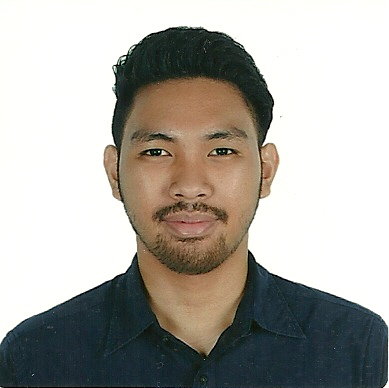
\includegraphics[width=0.2\columnwidth]{dan}
\documentAuthor{firstname2} \ \documentAuthor{surname2} is currently pursuing Bachelor of Science Degree in Computer Engineering at De La Salle University-Manila. His role in the group is the Master Programmer. With his adept skills in computer programming, he functions as the brain of the project, as he provides the main idea along with its purpose it serves. His research interests include mountaineering, agriculture, and robotics.

\vfill
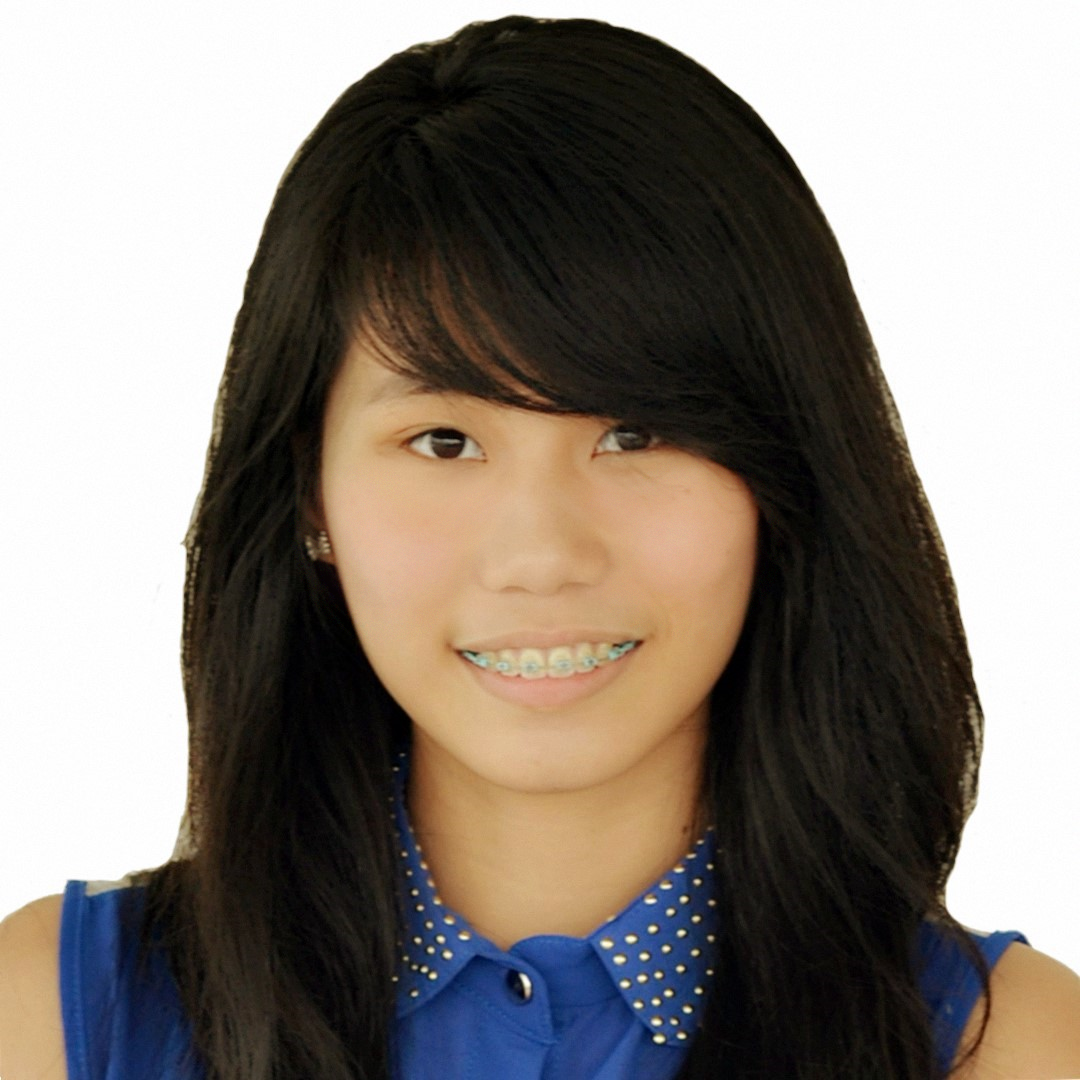
\includegraphics[width=0.2\columnwidth]{kath}
\documentAuthor{firstname3} \ \documentAuthor{surname3} is currently pursuing Bachelor of Science Degree in Computer Engineering at De La Salle University-Manila. With her keen sight for details, she provides constructive criticisms as to where the group will set rooms for further improvements and necessary corrections from established ideas. Her research interest include biomedical engineering, nanotechnology, and energy management systems.




\vfill
%}
\fi
\cleardoublepage

%%%%%%%%%%%%%%%%%%%%%%%%%%%%%%%%%%%%%%%%%%%%%%%%
\ifIndex
	\printindex
\fi
\cleardoublepage

\end{document}
